

\begin{frame}{ \textbf{Example  Importation à partir de fichiers JSON}}
\textbf{fichiers JSON}
       \begin{tabular}{cl}  
         \begin{tabular}{c}
           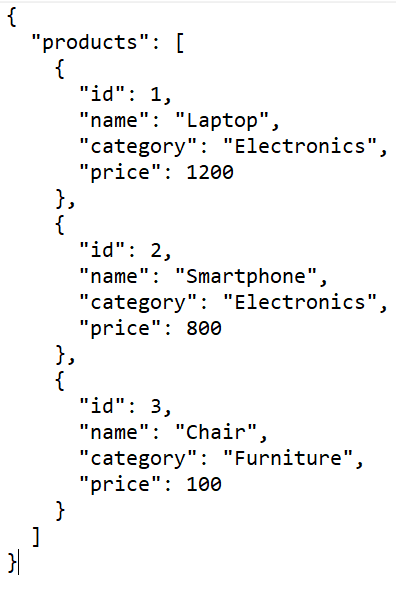
\includegraphics[height=4cm, width=3.5cm]{Frames/Travailler_avec_les_Données_dans_Neo4j/Capture.PNG}
           
           \end{tabular}
           & \begin{tabular}{l}
             \parbox{0.5\linewidth}{%  change the parbox width as appropiate
              
    }
         \end{tabular}  \\
\end{tabular}
 \begin{block}{\textbf{cypher} }
CALL apoc.load.json("file:///products.json") YIELD value
UNWIND value.products AS product
MERGE (p:Product {id: product.id})
SET p.name = product.name,
    p.category = product.category,
    p.price = product.price;

  \end{block}
    \end{frame}